\documentclass[12pt, a4paper]{article}

\usepackage[english]{babel}
\usepackage[utf8]{inputenc}

% Skip to next paragraph on whiteline
\usepackage{parskip}

% Define bounds where text can be drawn
%\usepackage[top=100pt,bottom=100pt,left=75pt,right=75pt]{geometry}

% Headings
\usepackage{fancyhdr}
\pagestyle{fancy}
\fancyhf{}
\lhead{Research Playa Printer}
\rfoot{Page \thepage}

% Colors and links
\usepackage{color}
\definecolor{blue}{rgb}{0,0.5,1}
\usepackage{hyperref}
\hypersetup{
	colorlinks = true,
	linkcolor = blue,
	urlcolor = blue,
	citecolor = blue,
}

% Enable images
\usepackage{graphicx}
\usepackage{float}
\graphicspath{{images}{../images/}}

% Bibliography package
\usepackage[numberedbib]{apacite}
\bibliographystyle{apacite}

% Load LaTeX subfiles
\usepackage{import}
\usepackage{subfiles}
\usepackage[subpreambles=true]{standalone}

% Titlepage
\title{\textbf{Research paper Playa Printer\\Project 7/8}}
\author{Stan Boer, 0931006}
\date{\today}

%Examples:
%This is an example citation \cite{example}

\begin{document}
	\clearpage
	\maketitle
	\thispagestyle{empty}
	\newpage

	\setcounter{page}{1}
	\newpage
	
\section{Summary}
The aim of this research paper is to take a closer look at the options to automate the process of mixing clay and supplying that to our 3D printer. This to eradicate the manual labour and constant monitoring required for operating the printer.

To look at our available options, we'll take a look at what other companies, such as WASP and Italian inventor Enrico Dini, have accomplished in the process of building their own printers. Community made printers are based on manually mixing their materials and putting those in containers, so this is something that will not be covered in this research.

At the end of this paper we will elaborate on our findings, and explain why our goal is not achievable within our current scope.
	\newpage
	
	\tableofcontents
	\newpage
	
\section{Introduction}
The initial goal for the project is to build a 3D printer which will be able to print with a mixture that consists out of sand and a form of glue or epoxy, the Playa Printer. The plan with the current prototype is to print with a self-made clay mixture, as this is the most accessible to us. This mixture has to be made either by hand or be mixed by a machine. This second option would eliminate the effort required to mix the clay ourselves. This machine is supposed to be constantly running, getting the clay mixture ready to be transported to the extruder. This will eliminate the need to manually refill the printer every time the extruder is out of clay.

As this is a far more convenient option for a printer of our scale, we'll be looking into options on how to tackle this idea. This research paper will cover what options there are, show research done on the subject and a conclusion in which we will decide what prototype to build.
\begin{figure}[H]
	\centering
	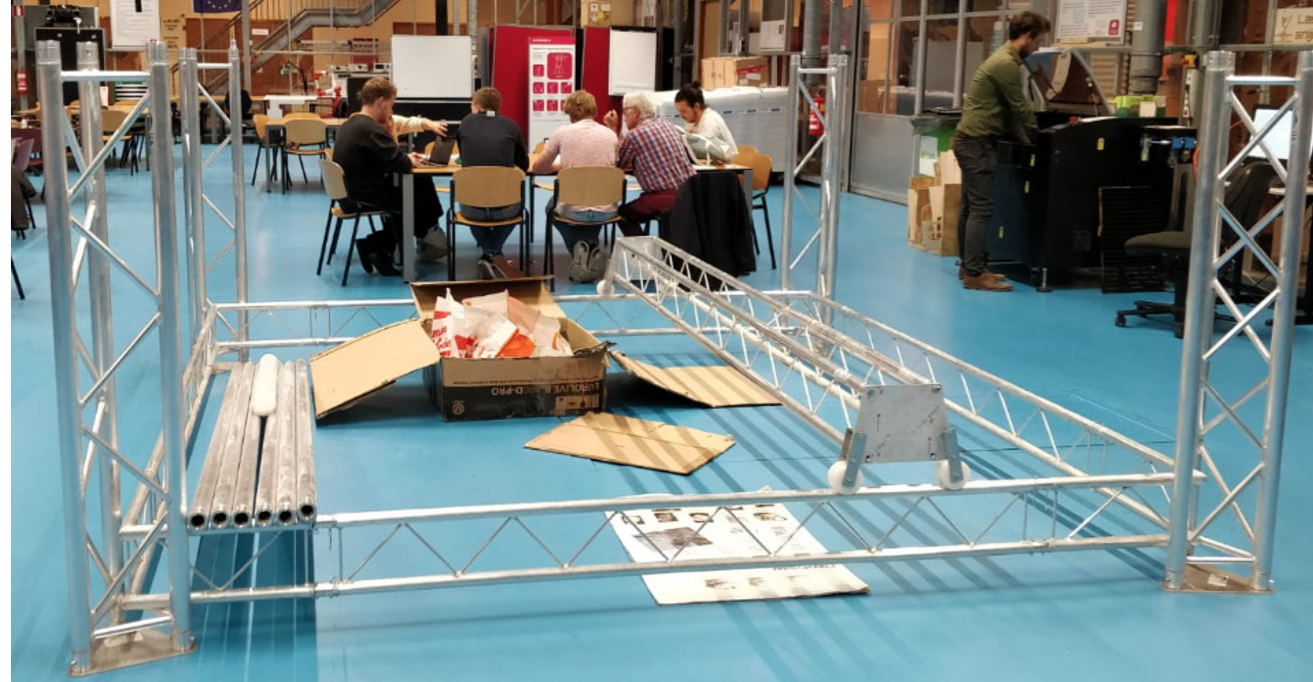
\includegraphics[width=14cm,height=14cm,keepaspectratio]{playaprinter}
	\caption{Playa Printer}
\end{figure}
	\newpage

\section{Research}
As the size of the printer is 3 by 3 meters, we will be needing a lot of material to be able to print at a scale like that. With existing 3D sand printers, the current method is to fill containers with the required mixture to be able to print with, and replace it every time the container is empty. For our project this can become quite inconvenient, which is why we will look in to figuring out a way of making this process more accessible. 
	
A company which created a similar 3D printer to ours, is called WASP. (reference) They created the Big Delta 3D printer, designed to be able to print with locally available materials at low cost. Their materials include mud combined with straw, and they are looking into the option to print with clay. They use a pugmill to combine their materials to be used as filament. When the extruder is empty, by the looks of it, the material has to be manually put into the extruder so that it can print again.
	
Unfortunately, there aren't any other companies working on a 3D printer of this scale. There are quite a few community made clay printers on small scale, so we can use that as a resource. Our aim will be to find a way to automatically mix our material together, and preferably pushes that to the extruder without requiring manual labour. The only effort required is to keep refilling the materials for the mixer. This situation would be close to ideal compared to what we are aiming for.

\section{Methodology}
Since 3D printing is picking up a lot of popularity, a lot more resources are available to us to develop a system on our down. To start, we'll have to look in to a different options on how to automate our mixing. Secondly, we'll have to compare the options, and pick one which we'll design a prototype for. 

To do an available product analysis, we'll be looking at the Big Delta printer from WASP and other companies who have attempted printing with sand. As the Big Delta printer is quite similar in design, it can be helpful in deciding our path to take. We'll be putting more priority on this specific printer than the other options. This will later be elaborated in the results.
	\newpage

\section{Results}
\subsection{Types of mixers}
\textbf{Hopper mixer}

Hopper mixers are an adaptation to mixers used for dough mixing, which consists of a horizontal shaft and either an open or lidded hopper. With this kind of mixer, dry material has to be added first and the liquid second. Some of thse mixers have the option to reverse the direction of the blades, so complete mixing can be achieved. Afterwards, the mixed clay has to be removed by hand and put in to the extruder.
\begin{figure}[H]
	\centering
	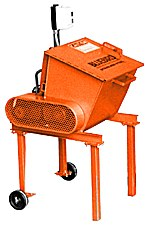
\includegraphics[height=10cm, keepaspectratio]{hoppermixer}
	\caption{Hopper mixer}
\end{figure}
	\newpage

\textbf{Soldner mixer}

Another form of mixers is a Soldner mixer, named after its designer. This mixer consists of a chain-driven rotating tub, with stationary bars on the inside, which allows the mixture to blend quickly and effectively. With this mixer it's normal to add the liquid first. After the dry material is added, it will be rotated through the stationary bars which chops and blends the clay for the desired consistency. This mixer also requires the material to be unloaded manually by hand and then stored.
\begin{figure}[H]
	\centering
	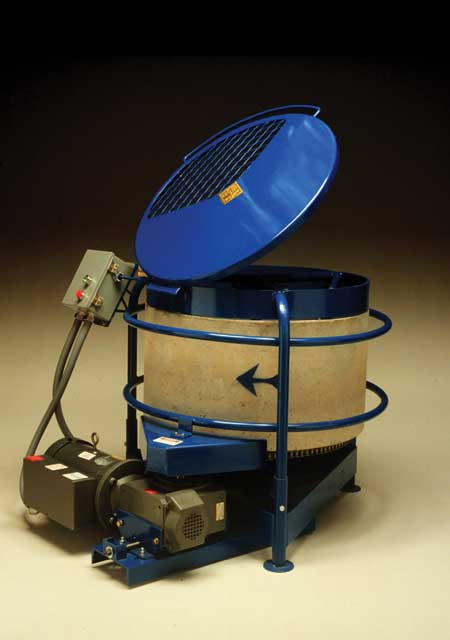
\includegraphics[height=12cm, keepaspectratio]{soldnermixer}
	\caption{Soldner mixer}
\end{figure}
	\newpage

\textbf{Pugmill}

Pugmills also work through a hopper and make use of a horizontal bladed shaft. The pugmill mixer requires moist clay to be put into the hopper which after blending gets extruded to a restricted opening at the end of a barrel. That means we are required to mix our material beforehand, which defeats the purpose of automating our process. Pugmills have the option to be equipped with a de-airing vacuum that can produce clay that is ready to be used, so that does give us an option of automation at the end of the process. 
\begin{figure}[H]
	\centering
	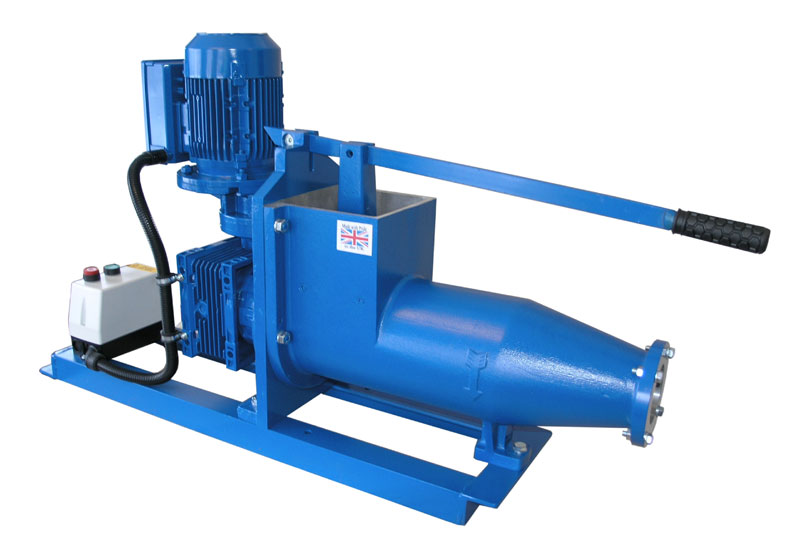
\includegraphics[width=12cm, keepaspectratio]{pugmill}
	\caption{Pugmill}
\end{figure}
	\newpage

\textbf{Mixer/pugmill}

Mixer/Pugmill combinations allow for both mixing clay and having a separate extruder for the material. The pugmill portion can serve as a discharge unit for the mixer, or as a separate pugmill on its own. The option of having a de-airing accessory will make it easier for us to automate the process of refilling the extruder.
\begin{figure}[H]
	\centering
	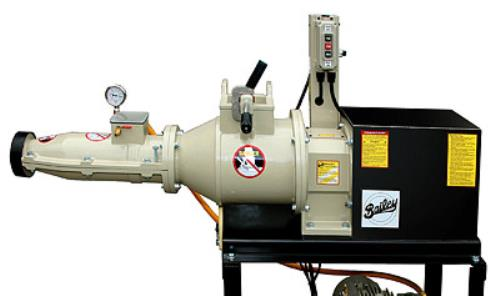
\includegraphics[width=12cm, keepaspectratio]{pugmixer}
	\caption{Mixer/pugmill combination}
\end{figure}
	\newpage

\subsection{Available printers}
To compare our available options, it is smart to look at what methods other companies use for their printers. Since there are only a few companies to look at, and most of them dont have their own resources available to us, our resources are quite limited to what we can find.

\textbf{Big Delta}

For our first example we will be looking at the Big Delta printer from WASP. They have built a 12 meter high printer, which they can use to print from locally available materials at low cost. Not much is known about their extruder. What is known just from pictures and videos from their demonstrations, is that they make use of an older pugmill. This mixer requires materials to be added to the machine, where it just keeps mixing the materials together untill it's ready for the extruder. It is also shown that the extruder needs to be manually refilled everytime, which can be quite some effort considering how high the printer can go.
\begin{figure}[H]
	\centering
	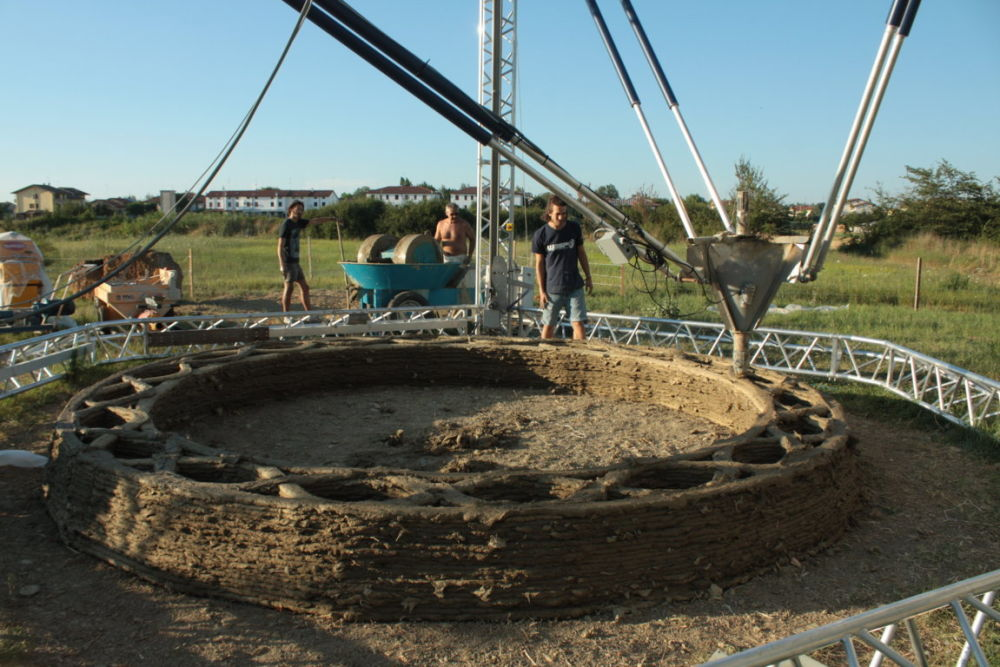
\includegraphics[width=11cm, keepaspectratio]{bigdelta}
	\caption{Big Delta printer using an older pugmill}
\end{figure}

This means that using an old hopmill and refilling manually still remaings one of our options, which is not really what we are looking for. It is unfortunate that they haven't gone towards automating this process, but this might still be a possibility for one of their future designs.
	\newpage
	
\textbf{D-Shape}
	
The D-Shape is a different kind of printer used than what we are working towards. This printer is effectively an up-scaled binder jetting process, where a binding material is dropped on each layer of powdered material. This method of printing is quite different than most orthodox 3D printers these days, is not really commercially available and would require us to completely rebuild our printer from scratch.
\begin{figure}[H]
	\centering
	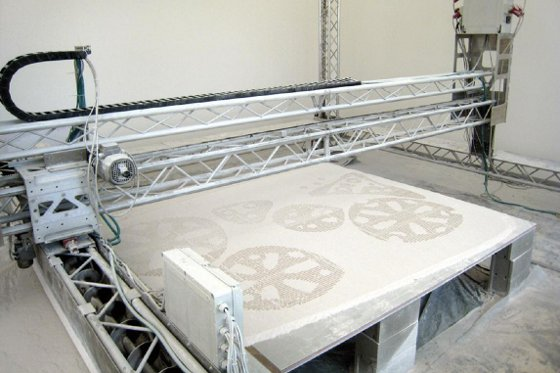
\includegraphics[width=11cm, keepaspectratio]{dshape}
	\caption{D-Shape printer}
\end{figure}

Even though the frame is a lot more similar to our design compared to the Big Delta printer, the concept used for this printer is unfortunately not an option for us. The way this printer is controlled might be a point of interest for us, but for the sake of this research we will not be looking deeper into this. Development on the D-Shape has not been progressing a whole lot from what we know, so it's not worth to continue spending time on this printer for now.
	\newpage

\subsection{Comparison}
Now that we have our options listed and given a brief overview of what every mixer is capable of, it's time to put this in a morphological chart. This will help us in deciding which machine works best for our prototype. Since it is of no importance to us if we make use of a horizontal or vertical mixing shaft, we'll be leaving this out of our chart.

Because there are not really any available solutions for us to automate this process, we will have to come up with something ourselves based on the information gathered. That's why we'll only be looking at the side of automating our mixing process.

	\begin{tabular}{ | p{3.2cm} || p{2cm} | p{2cm} | p{2cm}| p{2.6cm} | }
	\hline
	\multicolumn{5}{|c|}{\textbf{Morphological chart}} \\
	\hline
	\textbf{Type} & Hopper mixer& Soldner mixer & Pugmill & Mixer/Pugmill \\
	\hline
	\textbf{Material} & Dry/ Wet & Dry/ Wet & Wet only & Dry/ Wet \\
	\hline
	\textbf{Starting price} & \$2,000  & \$6,000 & \$2,500 & \$5,000  \\
	\hline
	\textbf{De-airing} & No & No & Yes/No & Yes/No \\
	\hline
	\textbf{Unloading} & Manually & Manually & Manually/ Automatic & Manually/ Automatic \\ 
	\hline
	\end{tabular}

It remains quite difficult to make a proper comparison between our available options, as they are quite limited. We know that each one of these options gets the job done, but the focus remains on the unloading part. Preferably, we want the option to work with both dry and wet material, as we do not know beforehand what local materials are available. Any form of de-airing is welcome, as it will allow us to make the unloading and reloading into the extruder much more accessible.
	\newpage

\section{Conclusion}
Unfortunately, based on our research, the option to automatically refill containers is going to remain quite difficult. All of the available mixers still require manual unloading, while a few have the option to build an automatic system to refill on our own and attach it to the machine. Based on the scale of the printer and the scale of building such a system ourself, it is not smart to pursue this option for now. 

Since it is only the first protoype of this printer, it will become quite more difficult with the addition of a lot of moving parts, which can all influence the quality of the print and the weight of the printer itself. The option to manualy refill containers still remains, as the containers we use can be custom made with an adapter designed by ourselves. This should be done in combination with a de-airing unit, as this would immedietly get the material ready to be put into the containers.

Because of the price of these machines, it will be quite difficult for us to afford one. Our only options are that we either get one sponsored, or that we build one from scratch ourselves. Designing one would take a lot of research on its own, so it is best to pursue this at a later point in development if time permits.

No matter if we can get access to any of these mixers, or design one on our own, it is most advisable to look at a mixer/pugmill combination. A normal pugmill only works with wet material, which does not accomplish what we want to do. Both a hopper mixer and a Soldner mixer do not have the option of de-airing, which also defeats the purpose of our goal. Since we do not have a budget for buying one, we will start designing a prototype of a mixer/pugmill combination, to see what our options are and to see if we can accomplish the mixing on our own without having to make a huge investment.
	\newpage

	\nocite{*}
	\bibliography{main}
	\newpage

\end{document}
